\section{构造与析构}
在很多时候,每当我们需要定义一个对象时,我们就会给它提供初始化。在C++中,\textbf{构造函数(Constructor)}为我们提供了一种方便的初始化方法;而\textbf{析构函数(Destructor)}能够在一个对象的生存期结束前对其进行最后处理——尤其是动态内存回收。\par
STL中的 \lstinline@std::vector@, \lstinline@std::list@,以及非STL的 \lstinline@std::string@\footnote{\lstinline@std::string@ 虽然有很多与STL容器相似的特性,但它不是STL的一部分。}, \lstinline@std::valarray@ 等类模板的内部机制都是靠动态内存分配来实现的,所以我们才可以动态地改变它的大小。在这里,我们也不妨把刚才定义的 \lstinline@valarri@ 也改成用动态内存分配来实现。\par
\subsection*{构造函数}
构造函数是一种特殊的成员函数,可以为一个对象提供初始化信息。每当我们定义一个新的对象时,相应的构造函数就会被调用,从而为这个对象进行初始化。\par
在C++中,如果我们不自定义一个构造函数的话,编译器会为这个类自动生成一个默认构造函数(Default constructor)。一个平凡的默认构造函数\footnote{由编译器生成的默认构造函数,通常来说是平凡的;但是也有例外,不过我们现在还没碰到,读者亦不必深究。}会什么也不做;如果我们希望它做些什么,对成员进行何种初始化,那么我们就需要按照可能的需求,自行定义一些构造函数。\par
就以 \lstinline@valarray@ 为例,现在我们需要让它用指针和动态内存分配的方式来管理数据,所以我们可以把上一节中的函数定义改成这样(主要修改的是私有成员部分):
\begin{lstlisting}
class valarri {
public:
    //...构造函数和析构函数部分,待补充
    std::size_t size() { return _size; } //返回当前的存储量大小
    int max();
    int min();
    int sum(); //声明max, min和sum
    valarri operator+(const valarri&); //可以与数组相加
    valarri operator+(int); //可以与数相加
    int& operator[](int i) { return _arr[i]; } //可以以下标形式访问
    valarri& operator=(const valarri&); //可以赋值
    valarri& operator+=(const valarri&); //可以加之以数组
    valarri& operator+=(int); //可以加之以数
    friend valarri operator+(int, const valarri&); //可以以数加之
    friend std::istream& operator>>(std::istream&, valarri&); //需iostream库
    //...待补充
private:
    static const std::size_t MAX_SIZE {100000}; //可以允许的容量会很大
    std::size_t _cap; //此数组的容量(可变)
    std::size_t _size; //此数组的存储量
    int *_arr; //这里改成指针,以便将来使用动态内存分配
}; //private成员的顺序需要慎重考虑,详见下文
\end{lstlisting}
接下来我们向其中添加构造函数。\par
构造函数的名字要与类名保持一致,所以在这里我们要定义成 \lstinline@valarri@。构造函数不能拥有返回值\footnote{后文我们会讲到,构造函数的作用并不是``制造和返回一个新的对象'',这个对象实际上在构造函数调用之前就已经存在,并且作为隐藏参数传入构造函数中。},所以我们在定义时直接写它的名字,带上参数列表和函数体就行了。
\begin{lstlisting}
//声明
public:
    valarri(); //默认构造函数
//定义
valarri::valarri() {
    _arr = nullptr; //指针置空是好习惯
    _cap = _size = 0; //一开始的容量和存储量当然是0
}
\end{lstlisting}
当我们定义一个对象,并且不提供初始化,或者是提供了空的初始化时\footnote{未必。如果该类有接收 \lstinline@std::initializer_list@ 的构造函数,那么提供空初始化时将会调用该构造函数,而非默认构造函数。我们会在下文中讲到相关内容。},就会调用默认构造函数。
\begin{lstlisting}
    valarray arr1; //不提供初始化,将调用默认构造函数
    valarray arr2 {}; //提供空初始化,将调用默认构造函数
\end{lstlisting}\par
只有当我们没有定义任何构造函数时,编译器才会生成一个默认构造函数(为了不破坏``定义变量时必须调用构造函数''的规则)。只要我们定义了一个构造函数,编译器就不会为我们生成默认构造函数。这时,如果我们不提供默认构造函数的话,那么就会形成一个默认构造函数的空缺——也就意味着,这时我们必须要提供定义,不能再省略了。\par
如果读者还有印象的话,应该会记得,我们在上一节中每逢定义一个 \lstinline@valarri@ 对象时,即便不想提供任何初始化,也需要写成 \lstinline@valarri v{}@ 而不能写成 \lstinline@valarri v@,原因就在于,我们已经定义了一个构造函数,但没有定义默认构造函数,所以我们不能不提供初始化。解决方法也很简单,像刚才一样提供一个默认构造函数就行了。\par
心细的读者可能会发现另一个问题——我们使用 \lstinline@valarri v{}@ 为什么就行了呢?难道提供空初始化和不提供初始化有什么区别吗?\par
其实,问题的关键在于,这里的 \lstinline@valarri v{}@ 并不是像 \lstinline@int i{}@ 的空初始化那样;这个初始化实际上传入了一个 \lstinline@std::initializer_list<int>@ 类型的参数!如果不信,你可以试试 \lstinline@valarri v()@ 这种写法,它是不能通过编译的。\par
这就不得不谈到 \lstinline@std::initializer_list@ 了。它是一个类模板,可以存储一个常量数组\\(\lstinline@const T[N]@ 类型)。我们可以这样验证它的类型\footnote{这里走了一点曲线,先用 \lstinline@auto@ 来创建一个对象,再去判断这个对象的类型。这是因为花括号嵌套内容在C++中的解释有多种可能,单纯的 \lstinline@\{1,2,3\}@ 未必是个对象,所以直接用 \lstinline@decltype(\{1,2,3\})@ 是行不通的。}:
\begin{lstlisting}
//包含头文件initializer_list
    auto ilist = {1,2,3}; //auto会自动识别初始化内容的类型,并作为ilist的类型
    std::cout << std::is_same< //用std::is_same来判断类型
        decltype(ilist), //ilist的类型在此之前被自动识
        std::initializer_list<int>
    > ::value;
\end{lstlisting}
这里的 \lstinline@ilist@ 是一个常量数组,它的值不能改变,只能被读取。\par
我们不能用下标运算符来直接读取 \lstinline@initializer_list@ 对象的值,必须用迭代器加循环的方式逐个访问:
\begin{lstlisting}
    auto ilist = { 1,2,3 };
    for (auto it = std::begin(ilist); it != std::end(ilist); it++) //循环
        std::cout << *it << ' '; //it是一个迭代器,其作用类似于指针
\end{lstlisting}
这样就会输出\\\noindent\rule{\linewidth}{.2pt}\texttt{
1 2 3 
}\\\noindent\rule{\linewidth}{.2pt}\par
还有一种更简单的方法是用范围 \lstinline@for@ 循环,请读者参考下面\\\lstinline@valarri::valarri(const std::initializer_list<int>&)@ 的定义:
\begin{lstlisting}
//声明
public:
    valarri(const std::initializer_list<int>&); //接收一个初始化表作为参数
//定义
valarri::valarri(const std::initializer_list<int> &ilist) {
    _cap = ilist.size(); //初始化_cap为ilist的大小
    _arr = new int[_cap]; //分配_cap大小的空间,刚好装得下
    _size = 0; //_size从0开始
    for (int x : ilist) //范围for循环,遍历ilist中的每个数
        _arr[_size++] = x; //赋值,_size自增
    //循环结束后_size会与_cap相等
}
\end{lstlisting}\par
有了构造函数之后,我们就可以这样定义 \lstinline@valarri@ 类的对象了:
\begin{lstlisting}
    valarri arr1 ({1,2,3}); //直接初始化语法,用()内的数组{1,2,3}进行初始化
    valarri arr2 {{1,2,3}}; //统一初始化语法,用{}内的数组{1,2,3}进行初始化
    valarri arr3 {1,2,3}; //列表初始化语法,用数据1,2,3构成的数组进行初始化
    valarri arr4 ({}); //直接初始化语法,用()内的数组{}进行初始化,其中数组为空
    valarri arr5 {{}}; //统一初始化语法,用{}内的数组{}进行初始化,其中数组为空
    valarri arr6 {}; //列表初始化语法,用没有数据的空数组进行初始化
    //以上初始化全都调用valarri::valarri(const std::initializer_list<int>&)
    valarri arr7; //没有提供任何初始化,将调用默认构造函数valarri::valarri()
\end{lstlisting}
其中 \lstinline@arr1@, \lstinline@arr2@, \lstinline@arr3@ 的初始化方式有别,但效果相同;\lstinline@arr4@, \lstinline@arr5@, \lstinline@arr6@ 的初始化方式有别,但效果相同;至于 \lstinline@arr7@,它的效果就完全不同了。接下来我来讲解一下这七个初始化的异同。\par
\lstinline@arr1@ 和 \lstinline@arr4@ 的初始化语法都使用了圆括号,它的另一种替代语法是用等号。但是读者不要误会,这里的等号和``赋值''没有任何关系,它的真实含义是构造函数。
\begin{lstlisting}
    valarri arr1 = {1,2,3}; //直接初始化语法,用数组{1,2,3}进行初始化
    valarri arr4 = {}; //直接初始化语法,用数组{}进行初始化,其中数组为空
\end{lstlisting}\par
在直接初始化的情况下,圆括号内的部分,或者等号后的部分,会作为参数传递给相应的构造函数——在这里当然就是 \lstinline@valarray::valarray(const std::initializer_list<int>&)@。\par
在C++11以后,我们一般的建议是使用统一初始化语法,也就是把圆括号换成花括号,写成 \lstinline@arr2@ 和 \lstinline@arr5@ 那样的形式。这两个花括号的含义是不一样的,外层的花括号表示这是一个统一初始化,内层的花括号表示这是一个数组,它的元素就是花括号内部的那些。\par
而 \lstinline@arr3@ 的定义语法叫作列表初始化——我们在定义原始数组的时候就经常这么干:
\begin{lstlisting}
    int array[5] {1,2,3,4,5}; //这里用到的也是列表初始化
\end{lstlisting}
其中列表初始化中的所有数据都必须是同一类型的。\par
总之,\lstinline@arr2@ 与 \lstinline@arr3@ 的初始化方式不同,一个是统一初始化,一个是列表初始化,但是它们最后都是调用了同一个构造函数,并且实现效果相同。至于 \lstinline@arr7@,我们根本就没有提供初始化(所以说初始化写成 \lstinline@{}@ 和完全不写是不同的!)
\subsection*{``列表初始化''与``统一初始化''间的权衡}
\lstinline@std::string@ 类(作为 \lstinline@std::basic_string<char>@ 的别名)有一个构造函数是这样的(其中的 \lstinline@CharT@ 是 \lstinline@char@,\lstinline@size_type@ 是 \lstinline@std::size_t@,下同。至于 \lstinline@alloc@,我们不用管,反正都有默认值):
\begin{lstlisting}
basic_string(
    const CharT *s,
    size_type count,
    const Allocator &alloc = Allocator()
);
\end{lstlisting}
它的作用是:取 \lstinline@s@ 字符串的前 \lstinline@count@ 个字符,作为此 \lstinline@std::string@ 对象的内容。以下是一个测试例子:
\begin{lstlisting}
    std::string str1 {"cppHusky", 3};
    std::cout << str1; //将输出cpp
\end{lstlisting}
读者会发现,我们在这里用的是花括号,它是一种统一初始化语法。\par
还有一个构造函数是这样的:
\begin{lstlisting}
basic_string(
    std::initializer_list<CharT> ilist,
    const Allocator &alloc = Allocator()
);
\end{lstlisting}
它的作用是:接收一个 \lstinline@char@ 数组,进而把它们拼成本字符串。
\begin{lstlisting}
    std::string str2 {'c','p','p','H','u','s','k','y'};
    std::cout << str2; //将输出cppHusky
\end{lstlisting}
我们在这里用的也是花括号,它是一种列表初始化语法。\par
所以说,统一初始化语法和列表初始化语法都在使用``一个花括号套若干项(可以是零个,一个或多个)''的操作。因此万一它们之间存在冲突,会发生什么呢?这是我们不可回避的问题。\par
来看一个典型的歧义例子。\lstinline@std::string@ 类有一个构造函数是这样的:
\begin{lstlisting}
basic_string(
    size_type count,
    CharT ch,
    const Allocator &alloc = Allocator()
);
\end{lstlisting}
它的作用是:以 \lstinline@count@ 个 \lstinline@ch@ 字符相拼接,从而形成本字符串。
\begin{lstlisting}
    std::string str3 {33, '='}; //试图通过统一初始化调用(size_type, CharT)版本
    std::cout << str3; //但输出的内容却是!=
\end{lstlisting}
我们发现,这次的输出内容并没有按我们预想的那样,输出33个 \lstinline@=@ 来。\par
原因就在于,编译器把这个 \lstinline@{33, '='}@ 解读成了列表初始化,于是 \lstinline@33@ 被隐式类型转换成了 \lstinline@'!'@。为了解决这个问题,我们不得不用传统的直接初始化方式。
\begin{lstlisting}
    std::string str4 (33, '=');
    std::cout << str4; //将输出=================================
\end{lstlisting}
这样就合乎预期了。\par
那么我们在之前定义 \lstinline@str1@ 的时候为什么没有遇到过这个问题呢?这是因为,\lstinline@"cppHusky"@ 无法隐式类型转换成 \lstinline@char@ 型,所以编译器不会把这里的初始化语法视为列表初始化,而是统一初始化。\par
总结一下:\textbf{编译器会优先把使用花括号的初始化方法当作列表初始化,并可以为此进行隐式类型转换;但是,如果不能通过隐式类型转换匹配到任何一个构造函数,那么编译器就会把这种初始化当作是统一初始化。}\par
\subsection*{成员的初始化}
构造函数的作用是为这个类的对象提供初始化。但是``对象有初始化''并不意味着``这个对象的成员有初始化''。\par
读者可能会问:我写构造函数的目的不就是为了给它的成员提供初值吗?如果我不写构造函数,直接用默认构造函数的话,那么我定义的局部对象的成员就会得到不确定的初值;现在我写了构造函数,让它有了确定的初值,难道这还不叫``初始化''吗?\par
先别急,我们来回顾一下之前写过的构造函数,比如\\\lstinline@valarri::valarri(const std::initializer_list<int>&)@,然后我们就会发现,这里的每个成员获得``初值''的方式都是``赋值'',而不是真正意义上的``初始化''!
\begin{lstlisting}
valarri::valarri(const std::initializer_list<int> &ilist) {
    _cap = ilist.size(); //_cap通过赋值获得“初值”
    _arr = new int[_cap]; //_arr通过赋值获得“初值”
    _size = 0; //_size通过赋值获得“初值”
    for (int x : ilist)
        _arr[_size++] = x; //赋值,但这里改变的不是哪个成员,而是成员指向的内容
    //循环结束后_size变为与_cap相等的值,这又是一个“初值”
}
\end{lstlisting}
如果仔细思考,你就会发现,这些成员全都是在``赋值'',而不是``初始化''。什么叫初始化?初始化就是,\textbf{当一个对象/成员生存期开始的时候,就已经有了一个我们给定的值}。而对于 \lstinline@_cap@ 或 \lstinline@_arr@ 来说,它们生存期的开始要早于我们为它赋值。那么它们的初值是多少呢?我们并未指定——所以我才说,``对象有初始化''并不意味着``这个对象的成员有初始化''。\par
那么如何初始化它们呢?我们有两种方法:\textbf{成员初始化列表(Member initializer list, 初值列)}和\textbf{默认成员初始值(Default member initializer)}。而在实操上,我们可以把默认成员初始值当作是``默认初值列''。接下来的讲解也会顺着这个思路走。\par
\subsubsection*{初值列}
初值列应当写在构造函数的参数列表和函数体之间,以冒号开始,并以逗号隔开。初值可以用圆括号或者花括号套起来,但是不能用等号。\par
下面的例子是一个新的 \lstinline@valarri@ 构造函数:
\begin{lstlisting}
//声明
public:
    valarri(int, std::size_t); //声明部分不要写初值列
//定义
valarri::valarri(int n, std::size_t size) //将n重复size次,作为新数组
    :_cap {size}, //用一个冒号开始值列;每个成员的初始化用逗号隔开
    _arr {new int[_cap]}, //用new[]来初始化
    _size {0}
{
    for (; _size < _cap; _size++) //通过循环赋值
        _arr[_size] = n; //赋值,每个元素都赋成n
    //循环结束后_size会与_cap相等
}
\end{lstlisting}
需要提醒读者的是,初值列应该写在定义中,而不是写在声明中。\footnote{作为对比,函数的默认参数最好写在声明中,而不是写在定义中。读者不要搞混了。}\par
\textbf{成员初始化的顺序仅仅取决于成员声明的顺序},至于初值列的顺序,那就没有影响了。这可能会造成一些问题——比如说,\lstinline@_cap@ 与 \lstinline@_arr@ 的初始化之间就存在依赖关系,我们必须先初始化 \lstinline@_cap@ 然后才能正确地初始化 \lstinline@_arr@。这就要求我们在声明成员变量时,就要把 \lstinline@_cap@ 放在 \lstinline@_arr@ 之前(所幸,我们一开始的声明顺序就是正确的,所以我们不会遇到这些问题)。
\begin{lstlisting}
private:
    std::size_t _cap;
    std::size_t _size;
    int *_arr; //它的初始化依赖于_cap,所以必须置于_cap之后
\end{lstlisting}
同理,我们也可以把另外两个构造函数也用初值列语法改写一下:
\begin{lstlisting}
valarri::valarri() :_cap {0}, _arr{nullptr}, _size {0} 
    {}//函数体中不再需要做什么了,空着就行
valarri::valarri(const std::initializer_list<int> &ilist) 
    :_cap {ilist.size()},
    _arr {new int[_cap]},
    _szie {0}
{
    for (int x : ilist) //范围for循环,遍历ilist中的每个数
        _arr[_size++] = x; //赋值,_size自增
    //循环结束后_size会与_cap相等
}
\end{lstlisting}
\subsubsection*{默认成员初始值}
在写初值列时,我们发现,除去一些特殊情况(比如默认构造函数)外,好像 \lstinline@_arr@ 的初始化值都是 \lstinline@new int[_cap]@。为了简单一点,我们可以直接设置一个``默认初值'',这就是默认成员初始值。\par
默认成员初始值要在类的定义当中写。可以用等号、圆括号或者花括号。不过延续本书的一贯的习惯,我们还是选择使用花括号。
\begin{lstlisting}
private:
    std::size_t _cap {0}; //_cap的默认初值是0
    std::size_t _size {0}; //_size的默认初值是0
    int *_arr {new int[_cap]}; //_arr的默认初值为new int[_cap],它依赖于_cap
\end{lstlisting}\par
接下来我们就可以在此默认值的基础上,简化前面写过的三个构造函数:
\begin{lstlisting}
valarri::valarri(){} //默认初值正好合适,就不需要写多余代码了
valarri::valarri(const std::initializer_list<int>& ilist)
    :_cap {ilist.size()} //_cap的初值需要单独指定,其它成员的初值就不需要了
{
    for (int x : ilist) //范围for循环,遍历ilist中的每个数
        _arr[_size++] = x; //赋值,_size自增
}
valarri::valarri(int n, std::size_t size) :_cap {size} {
    for (; _size < _cap; _size++) //通过循环赋值
        _arr[_size] = n; //赋值,每个元素都赋成n
    //循环结束后_size会与_cap相等
}
\end{lstlisting}
这样一来,写初始化也可以事半功倍了。\par
\subsection*{析构函数}
一个对象一经定义,它就存在了;一经初值列,它的成员就有了初值;调用完构造函数,它的存在就有了意义\footnote{关于``对象的生存期''始自何时,不同人有不同见解。有些人认为,其生存期始自定义之时;也有人认为,其生存期始自构造函数调用完成之时。本书不打算在这个问题上多做文章。}。但是,无论这个对象的存储期是自动的、静态的,还是动态的,它总有存储期结束的那一刻。在生存期结束之前,它会调用析构函数——这是它安排后事最后的机会。\par
在C++中,如果我们没有自定义析构函数,那么编译器会创建一个``什么也不做''的析构函数。如果不需要什么特别安排的话,自带的析构函数足够用了,我们根本不需要自行定义。\par
然而在涉及动态内存分配的问题上,我们就有责任定义一个能够回收动态内存的析构函数,以防内存泄漏。动态内存既不是指针的一部分,也不是对象的一部分,不会自动回收,我们只能用 \lstinline@delete@/\lstinline@delete[]@ 来回收,而析构函数就是在这方面的最佳选择。\par
析构函数也是一种特殊的函数,它既不能有返回值,又不能接收任何参数,一般也不需要我们手动调用\footnote{一个例外是,布置分配的动态对象需要显式调用析构函数,否则可能发生内存泄漏。我们到了精讲篇再谈。}——析构函数会在对象生存期结束之前调用,调用完毕后对象的生存期立刻结束。\par
析构函数的名字是由一个波浪号加类名的形式写成的。它不可以重载,所以每个类只能有一个析构函数。
\begin{lstlisting}
//声明
public:
    ~valarri(); //析构函数
//定义
valarri::~valarri() {
    delete[] _arr; //回收_arr指向的动态内存空间,注意必须要用delete[]搭配
} //其它成员不用再改动,_arr也没必要指向nullptr,反正析构函数结束了它们都没了
\end{lstlisting}\par
析构函数为我们提供了极大的方便,我们不需要手动回收它申请的动态内存,也不用害怕忘记回收(任何一个非动态存储期对象,只要它的生存期结束,它就一定会先调用析构函数)。STL等类模板的内部实现全都要靠动态内存分配来实现,但我们不需要因此而为那么专属于动态内存分配的细节而感到头疼,只需要把 \lstinline@std::vector@ 或 \lstinline@std::string@ 类的对象当成自动/静态存储期的对象来使用就足够了。这正是封装的优点!\par
\subsection*{拷贝构造函数}
有些时候,我们需要用另一个对象来为某个对象初始化,也就是把另一个对象的值复制给新定义的对象。这种情况最常见于参数传递。当我们按值传递某个类的参数时,程序都会调用这个类的构造函数来为这个形参对象进行初始化——这种构造函数又叫\textbf{拷贝构造函数(Copy constructor)}。
\begin{lstlisting}
void fun(valarri a) { //在传递参数时会进行拷贝构造
    //...
}
\end{lstlisting}\par
如果我们没有自定义拷贝构造函数的话,编译器会为我们定义一个。如果我们只需要单纯地把一个对象的值复制一份给另一个对象,那么用自带的拷贝构造函数足够了。\par
有些时候我们不得不自定义拷贝构造函数。比如,在设计含有动态内存分配的类时,构造函数那种单纯的``值拷贝''有时并不是我们想要的。什么意思呢?\par
\subsubsection*{浅拷贝及其缺陷}
还以 \lstinline@valarri@ 为例。
\begin{lstlisting}
    valarri a {1,2,3,4}; //用列表初始化创建一个长度暂时为4的数组
    valarri b {a}; //用a来拷贝构造b
\end{lstlisting}
我们分析一下这个过程中会发生什么。其实很简单,\lstinline@b@ 的 \lstinline@_cap@ 私有成员将获得与 \lstinline@a@ 的 \lstinline@_cap@ 成员相同的值——其实我们也希望这样。\par
同样的道理,\lstinline@b._size@ 也将获得与 \lstinline@a._size@ 相同的值。这也是我们所希望的。\par
同理,\lstinline@b._arr@ 也将获得与 \lstinline@a._arr@ 相同的值。但是这里就有点耐人寻味了——\par
\lstinline@_arr@ 成员可是指针啊。如果它们指向同一段内存空间,这会意味着什么呢?会意味着,当我修改 \lstinline@a[0]@ 的时候,\lstinline@b[0]@ 也会跟着同步修改;会意味着,当我需要析构 \lstinline@a@ 但不想析构 \lstinline@b@ 的时候,\lstinline@a._arr@ 指向的内存空间被回收,而 \lstinline@b@ 指向的内存空间一样被回收了(因为它们指向的就是同一个内存空间)。\par
简单点说就是——你这算哪门子拷贝啊,你这压根就是没扯清关系的别名吧。\par
这种现象就是\textbf{浅拷贝(Shallow copy)},它的缺陷是:它只是单纯地进行``值''层面的复制;但是对于指针来说,我们需要复制的未必是指针的值(地址),而可能是指针指向内存空间中的内容。这时候自带的拷贝构造函数就无能为力了,因此我们需要自己写一个拷贝构造函数,以此解决这个问题。\par
\subsubsection*{深拷贝及其实现}
\textbf{深拷贝(Deep copy)}的特点在于,它不是复制地址而是复制内容。图8.2展示了它们之间的区别。
\begin{figure}[htbp]
    \centering
    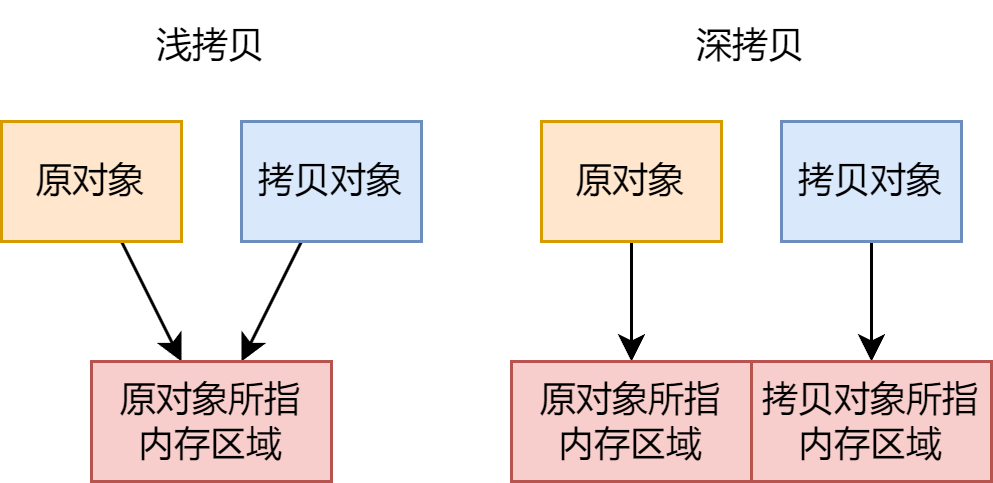
\includegraphics[width=0.8\textwidth]{../images/generalized_parts/08_shallow_copy_and_deep_copy.drawio.png}
    \caption{浅拷贝与深拷贝}
\end{figure}\par
要实现深拷贝其实很简单,就像一般的构造函数那样写就行了,只是参数类型变成了\\\lstinline@const valarri&@ 而已,剩下的只是按我们的需要复制值或内容而已。
\begin{lstlisting}
//声明
public:
    valarri(const valarri&); //拷贝构造函数
//定义
valarri::valarri(const valarri &a)
    :_cap{a._cap},
    _size{a._size},
    _arr{new int[_cap]} //_arr应指向自己独有的存储空间,而不是和a._arr一样
{ //(另:鉴于_arr的默认初值就是new int[_cap],所以这里可以省略这个初值)
    for (int i = 0; i < _size; i++)
        _arr[i] = a._arr[i]; //拷贝每个值,而不是拷贝地址
}
\end{lstlisting}\par
不止是拷贝构造函数,赋值运算符也必须自定义,从而防范发生``复制了地址而不是内容''的情况。不过赋值运算符相比于拷贝构造函数,还需要考虑更多东西才行。\par
首先是防止自我赋值。这个好说,按照老办法,检测一下 \lstinline@&a==this@ 就行了。\par
还有,这个对象的 \lstinline@_arr@ 成员指向的内存空间可能已经存储了一些值。这些值当然可以不管,但 \lstinline@_arr@ 指向的内存空间不能不管。怎么处理呢?如果我们需要赋值的数据太多,现有的容量装不下,那我们就得重新分配一个更大的内存空间了;如果需要赋值的数据不多,现有的容量足够装得下,那我们就直接装进去就好了。所以我们需要一个条件语句。\par
\begin{lstlisting}
valarri& valarri::operator=(const valarri &a) { //重载赋值运算符,防止浅拷贝
    if (&a == this) //防止自我赋值
        return *this;
    if (_cap < a._size) { //如果现有容量装不下a中的所有数据,那就要扩容
        delete[] _arr; //别忘了先回收现在指向的内存空间!!
        _cap = a._size; //_希望分配一个大小为a._size的内存空间
        _arr = new int[_cap]; //分配动态内存空间
    }
    for (_size = 0; _size < a._size; _size++)
        _arr[_size] = a._arr[_size]; //用循环语句复制内容
    return *this; //返回*this
}
\end{lstlisting}\par
我们在本节中修改了 \lstinline@valarri@ 的定义,包括但不限于添加了 \lstinline@_cap@ 成员,且把 \lstinline@_arr@ 成员由数组改成了指针。所以我们在第二节中写的很多函数也需要重新修改调整。本书没有余裕一一赘述,就请读者自行尝试吧。\par
